\documentclass[titlepage]{article}
\usepackage{xcolor}
\usepackage[english, croatian]{babel}

\usepackage{verbatim}
\usepackage{graphicx}
\usepackage{float}
\graphicspath{ {./Dijagrami_slike/} }

\title{INFORMACIONI SISTEMI\\Kovid sistem}
\author{
Bogdan Bojović 1019/2021\\
Kosta Grujčić 1012/2021\\
Miodrag Radojević 1012/2020\\
Luka Đorović 1029/2021\\
Irena Vasiljević 1018/2021
}

\date{Beograd, 2021.}

\begin{document}

\maketitle
\tableofcontents

\newpage

\section{Uvod}

\section{Analiza sistema}

Informacioni sistem Kovid centar svojim funkcionalnostima obezbe\dj{}uje sigurno i brzo sprovo\dj{}enje procedura neophodnih za za\v{s}titu od virusa COVID-19. Namenjen je pre svega osobama koje nameravaju da se testiraju i/ili vakcini\v{s}u kao i nadle\v{z}nim licima za kori\v{s}\'{c}enje relevantnih statistika.\newline
\indent Rezultati testova, informacije o testiranim licima, informacije o vakcinisanim licima i drugo, predstavljaju podatke koje na\v{s} informacioni sistem koristi pri a\v{z}uriranju korisnika o narednim koracima za\v{s}tite od virusa kao i pri dodeljivanju kovid propusnica. Pored toga, na zahtev mo\v{z}emo podatke dostaviti nadle\v{z}nim licima iz ministarstva zdravlja.\newline
\indent Na Slici \ref{slk:slucajevi} nalazi se dijagram koji prikazuje učesnike sistema i njihove poslove.

\begin{figure}[H]
\centering
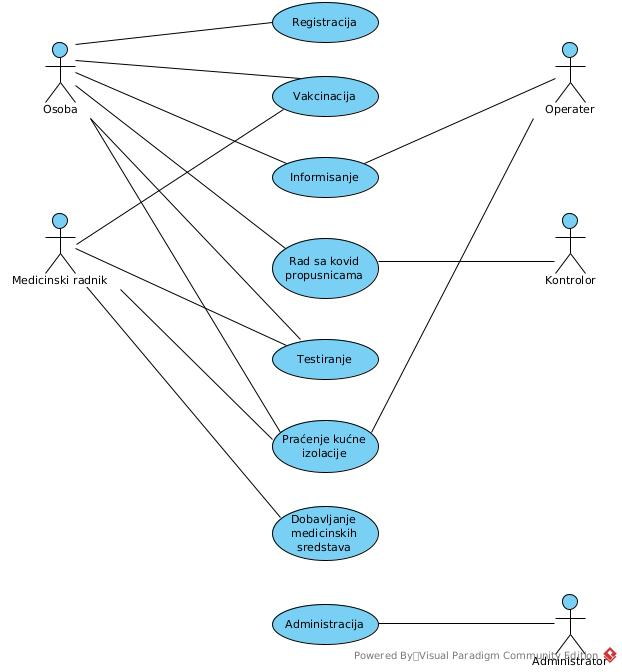
\includegraphics[scale=0.5]{Dijagram_slucajeva_upotrebe}
\caption{Dijagram slučajeva upotrebe}
\label{slk:slucajevi}
\end{figure}


\section{Procesi i slučajevi upotrebe}

%Menjajte strukturu i nazive kako vam se uklapa u slučaj :)

\subsection{Prva doza vakcine - aktivnosti}
Ovo poglavlje sačinjeno je od formalno predstavljenih slučajeva upotrebe počev od podnošenja prijave do evidentiranja uspešno primljene prve doze vakcine.

\subsubsection{Sličaj upotrebe: Online registracija}
\begin{itemize}
    \item \textbf{Kratak opis:} Neregistrovana osoba vrši registraciju popunjavanjem online forme, traženim podacima. Sistem potvrđuje validnost podataka i vraća potvrdu o uspešnosti registracije.
    \item \textbf{Učesnici:}
        \begin{itemize}
            \item Neregistrovana osoba - želi da se registruje u sistem, u cilju podnošenja zahteva za vakcinaciju.
        \end{itemize}
    \item \textbf{Preduslovi:} Sistem je aktivan. Neregistrovana osoba ima pristup internetu.
    \item \textbf{Postuslovi:} Osoba je registrovana i ima pristup sistemu. Njeni podaci su sačuvani u bazi. Dobila je korisničko ime i lozinku uz pomoć kojih se loguje na sistem.
    \item \textbf{Osnovni tok:}
        \begin{enumerate}
            \item Osoba otvara web-stranicu za registraciju.
	    \item Sistem prikazuje formular za registraciju.
	    \item Osoba unosi tražene podatke.
	    \item Osoba potvrđuje unos.
	    \item Sistem vrši validaciju podataka.
	    \item Sistem čuva podatke.
	    \item Sistem pravi privremeni nalog.
	    \item Sistem šalje osobi email u kojem traži potvrdu registracije.
	    \item Sistem obaveštava osobu da je email poslat.
	    \item Osoba proverava poštu i potvrđuje registraciju.
	    \item Sistem privremeni nalog trajno aktivira.
            \item Sistem obaveštava osobu da je uspešno registrovana.
	\end{enumerate}
     
    %Ako postoje, podtokove nazivati sa P1, P2, ...   
    %\item \textbf{Podtokovi:}    
    
    %Alternativne tokove nazivati sa A1, A2, ...
    \item \textbf{Alternativni tokovi:}
        \begin{itemize}
            \item[A1.] \textbf{Neuspešna validacija podataka.} Ukoliko u koraku 5 osnovnog toka sistem naiđe na neispravne podatke, obaveštava korisnika i zahteva ponovni unos onih polja gde su nevalidni podaci. Pri čemu označava korisniku polja sa nevalidnim podacima. Kada osoba unese sve podatke ispravno, proces se nastavlja u koraku 4 osnovnog toka.
            \item[A2.] \textbf{Nije stigao email za potvrdu registracije.} Ukoliko osoba nije dobila email za potvrdu, klikom na dugme zahteva ponovno slanje emaila. Proces se nastavlja u koraku 8.
	    \item[A3.] \textbf{Link za registraciju je istekao.} Ukoliko osoba nije potvrdila registraciju u predviđenom periodu, sistem briše privremeni nalog. Proces se završava.
        \end{itemize}
    
    %Ako postoje, specijalne zahteve navesti ovde
    \item \textbf{Specijalni zahtevi:}
		\begin{itemize}
			\item Potrebno je da je osoba koja se registruje punoletna.
		\end{itemize}
  
    \item \textbf{Dodatne informacije:}
        \begin{itemize}
            \item  Podaci potrebni za prijavu su:
                \begin{itemize}
                    \item ime
                    \item prezime
                    \item JMBG
                    \item broj zdravstvene knjižice
                    \item broj telefona
                    \item email adresa
		    \item korisničko ime
		    \item lozinka
                \end{itemize}
        \end{itemize}

\end{itemize}


\subsubsection{Slučaj upotrebe: Podnošenje prijave online}
\begin{itemize}
    \item \textbf{Kratak opis:} Neprijavljena osoba vrši prijavu popunjavanjem online forme, traženim podacima. Sistem potvrđuje validnost podataka i vraća poruku o uspešnosti prijave.
    \item \textbf{Učesnici:}
        \begin{itemize}
            \item Neprijavljena osoba - želi da se prijavi za prvu dozu vakcine.
        \end{itemize}
    \item \textbf{Preduslovi:} Sistem je aktivan. Neprijavljena osoba je registorvana kao korisnik sistema i ima pristup internetu.
    \item \textbf{Postuslovi:} Korisnik je dobio potvrdu o zakazanom terminu i mestu prve vakcinacije.
    \item \textbf{Osnovni tok:}
        \begin{enumerate}
            \item Osoba otvara web-stranicu za logovanje.
	    \item Osoba unosi i potvrđuje korisničko ime i lozinku.
            \item Sistem prikazuje formular za prijavu.
            \item Osoba bira ponuđeno vreme i proizvođače vakcina.
            \item Osoba potvrđuje unos.
            \item Sistem čuva unete podatke.
	    \item Sistem daje mogućnost izbora raspoloživih ustanova za zadat termin i vakcine.
	    \item Osoba bira ponuđene ustanove i potvrđuje. 
            \item Sistem zakazuje termin vakcinacije.
	    \item Sistem korisniku šalje email sa potvrdom o zakazanom terminu.
            \item Sistem obaveštava korisnika da je operacija uspešno izvršena i da je potvrda poslata.
	\end{enumerate}
     
    %Ako postoje, podtokove nazivati sa P1, P2, ...   
    %\item \textbf{Podtokovi:}    
    
    %Alternativne tokove nazivati sa A1, A2, ...
    \item \textbf{Alternativni tokovi:}
        \begin{itemize}
            \item[A1.] \textbf{Neuspešno logovanje.} Ukoliko u koraku 2 osnovnog toka sistem naiđe na neispravne podatke, obaveštava korisnika i zahteva ponovni unos korisničkog imena i lozinke. Proces se nastavlja u koraku 2 osnovnog toka.
        \end{itemize}
    
    %Ako postoje, specijalne zahteve navesti ovde
    \item \textbf{Specijalni zahtevi:}
		\begin{itemize}
			\item Potrebno je da je zdravstvena knjižica, osobe koja zakazuje vakcinaciju, u trenutku zakazivanja važeća.
		\end{itemize}
  
\end{itemize}

\begin{figure}[H]
\centering
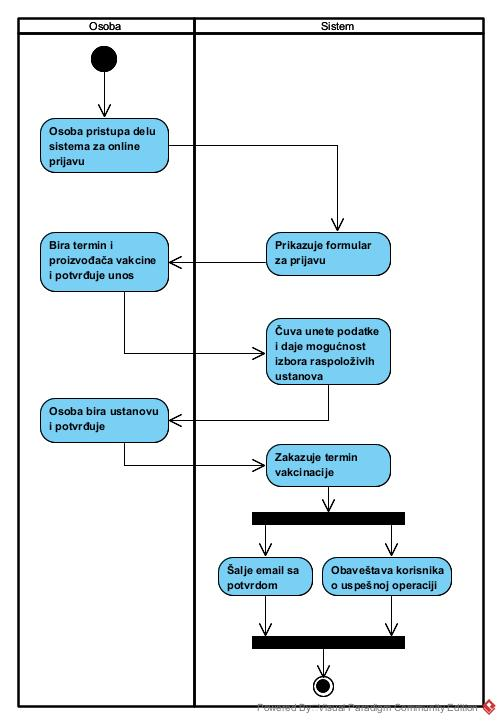
\includegraphics[scale=0.7]{Podnosenje_prijave_online}
\caption{Dijagram aktivnosti - Pondnošenje prijave online}
\end{figure}


\subsubsection{Slučaj upotrebe: Podnošenje prijave uživo}
%\subsubsection{Slučaj upotrebe: Evidentiranje prijave u sistemu}
\subsubsection{Slučaj upotrebe: Obaveštavanje o terminu vakcinacije online}
\subsubsection{Slučaj upotrebe: Obaveštavanje o terminu vakcinacije uživo}
\subsubsection{Slučaj upotrebe: Otkazivanje termina vakcinacije}
%\subsubsection{Slučaj upotrebe: Izadavanje online potvrde o vakcinaciji}
%\subsubsection{Slučaj upotrebe: Izdavanje uživo potvrde o vakcinaciji}


\subsection{Obaveštavanje o drugoj/trećoj dozi vakcine}
\subsubsection{Slučaj upotrebe: Obave\v{s}tavanje o drugoj dozi vakcine}
\begin{itemize}
    \item \textbf{Kratak opis:} Sistem na osnovu podataka o prvom primanju vakcine vakcinisanoj osobi \v{s}alje obave\v{s}tenje o primanju druge doze (mesec dana nakon primanja prve).
    \item \textbf{Učesnici:} 
        \begin{itemize}
            \item Vakcinisana osoba.
        \end{itemize}
    \item \textbf{Preduslovi:} Sistem je aktivan, podaci o vakcinaciji osobe su a\v{z}urirani.
    \item \textbf{Postuslovi:} Оsoba dobija podatke o vremenu i mestu vakcinacije. Sistem je a\v{z}uriran. 
    \item \textbf{Osnovni tok:}
    \begin{enumerate}
        \item Sistem pristupa podacima o vakcinisanima.
        \item Sistem predla\v{z}e vreme i mesto vakcinacije drugom dozom vakcine koja je već primljena prvi put.
        \item Osoba prihvata vreme i mesto vakcinacije.
        \item Sistem obave\v{s}tava osobu da je termin zakazan.
        \item Sistem a\v{z}urira podatke o zakazanim terminima.
    \end{enumerate}
    \item \textbf{Alternativni tokovi:}
    \begin{itemize}
        \item[A1.] \textbf{Osoba ne prihvata predlo\v{z}eni termin.} Ukoliko osoba nije u mogućnosti da zadovolji predlo\v{z}eni termin, sistem to uva\v{z}ava i prosle\dj{}uje formular u kome osoba zadaje vreme i mesto vakcinacije. 
        \item[A2.] \textbf{Sistem ne prihvata zadati termin.} Ako sistem ne prihvata zadati termin, \v{s}alje isti formular osobi. Ukoliko sistem prihvati zadato, proces se nastavlja u ta\v{c}ki 4 osnovnog toka.
        
    \end{itemize}
    \item \textbf{Dodatne informacije:}
    \begin{itemize}
        \item Sistem treba ponuditi mogućnosti osobi koja želi da popuni formular, u vidu spiska lokacija Kovid-ambulanti i spiska termina (datum i vreme - na svakih pola sata u okviru radnog vremena).
    \end{itemize}
\end{itemize}


\begin{figure}[H]
\centering
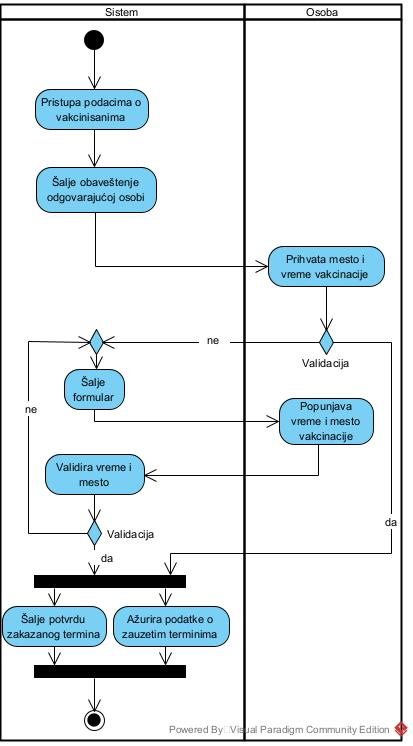
\includegraphics[scale=0.8]{Vakcinacija_drugom_dozom}
\caption{Dijagram aktivnosti - Obaveštavanje o vakcinaciji drugom dozom}
\end{figure}


\subsection{Informisanje}
\subsubsection{Slučaj upotrebe: Sprovođenje statistike nadle\v{z}nom licu}
\begin{itemize}
\item \textbf{Kratak opis:}  Nadle\v{z}no lice iz ministarstva zdravlja popunjava formular na osnovu kojeg mu se nakon autentikacije i konsultovanja baze podataka u malom broju koraka dostavljaju tra\v{z}eni podaci.
\item \textbf{Učesnici:}
\begin{itemize}
    \item Nadle\v{z}no lice iz ministarstva iz zdravlja.
\end{itemize}
 \item \textbf{Preduslovi:} Sistem je aktivan. Potra\v{z}ilac statistike iz ministarstva zdravlja ima pristup internetu.
 \item \textbf{Postuslovi:} Ministarstvu su na raspolaganje dostavljeni zatra\v{z}eni podaci.
 \item \textbf{Osnovni tok:}
 \begin{enumerate}
    \item Lice iz ministarstva otvara stranicu za autentikaciju.
    \item Sistem prikazuje formular za autentikaciju.
    \item Lice iz ministarstva popunjava polja za: ime, prezime, JMBG i jedinstveni identifikacioni broj koji je specijalno dodeljen za ovaj vid transakcije.
    \item Lice potvrđuje unos.
    \item Sistem proverava informacije koje su mu dostavljene u popunjenom formularu za autentikaciju.
    \item Nakon provere identiteta, sistem obave\v{s}tava lice iz ministarstva o uspe\v{s}nosti autentikacije.
    \item Sistem prikazuje stranicu sa ponu\dj{}enim opcijama za dohvatanje statistike.
    \item Lice iz ministarstva bira neke od opcija:
    \begin{itemize}
                    \item Dohvatanje statistike o broju vakcinisanih Pfizer-BioNTech vakcinom u odre\dj{}enom vremenskom periodu.
                    \item Dohvatanje statistike o broju vakcinisanih Sputnik V vakcinom u odre\dj{}enom vremenskom periodu.
                    \item Dohvatanje statistike o broju vakcinisanih Sinopharm vakcinom u odre\dj{}enom vremenskom periodu.
                    \item Dohvatanje statistike o broju vakcinisanih Oxford/AstraZeneca vakcinom u odre\dj{}enom vremenskom periodu.
                    \item Dohvatanje statistike o broju testiranih na COVID-19 u odre\dj{}enom vremenskom periodu.
                    \item Dohvatanje statistike o broju osoba sa pozitivnim testom na \newline COVID-19 u odre\dj{}enom vremenskom periodu.
                    \item Dohvatanje informacija (vreme, identitet lica iz ministarstva) o prethodnim potra\v{z}ivanjima iz ministarstva zdravlja.
                \end{itemize}
    \item Sistem proverava da li je uspe\v{s}no izabrana neka od opcija.
    \item Sistem na osnovu izbora dostavlja statistiku licu iz ministartstva zdravlja.
    \item Informacije o vremenu i identitetu potra\v{z}ioca \v{c}uvaju se u sistemu.
 \end{enumerate}
 \item \textbf{Alternativni tokovi:}
 \begin{itemize}
            \item[A1.] \textbf{Neuspe\v{s}na dodela dozvole za podno\v{s}eje zahteva.} Ukoliko u koraku 5 osnovnog toka sistem naiđe na neispravne podatke, obaveštava korisnika i zahteva ponovni unos podataka. Proces se nastavlja u koraku 3 osnovnog toka.
            \item[A2.] \textbf{Neispravno podno\v{s}enje zahteva.} Ukoliko u koraku 9 osnovnog toka sistem utvrdi da lice iz ministarstva nije odabralo nijednu od ponu\dj{}enih opcija, lice o tome biva obave\v{s}teno. Proces se nastavlja u koraku 8 osnovnog toka. 
        \end{itemize}
 \item \textbf{Dodatne informacije:}
            \begin{itemize}
                \item Jedinstveni identifikacioni broj koji se koristi za autentikaciju u\v{c}esnika i dodelu dozvole za podno\v{s}enje zahteva za statistiku dodeljuje se u dogovoru sa ministarstvom zdravlja posebno svim licima koja \'{c}e biti  zadu\v{z}ena za dohvatatanje statistike.
            \end{itemize}

\end{itemize}

\begin{figure}[H]
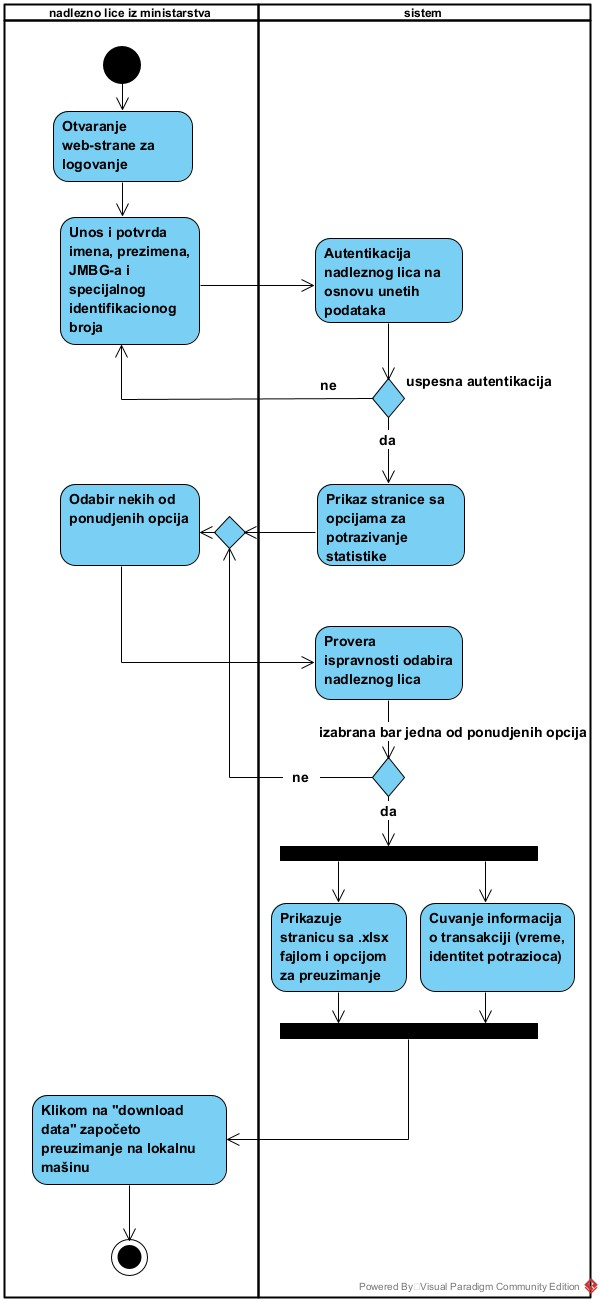
\includegraphics[scale=0.53]{Sprovodjenje_statistike}
\caption{Dijagram aktivnosti - Sprovo\dj{}enje statistike nadle\v{z}nom licu}
\end{figure}

\subsubsection{Slučaj upotrebe: Kol centar}
\begin{itemize}
\item \textbf{Kratak opis:} Osoba poziva kol centar Kovid sistema u cilju informisanja. Dodeljenom opereteru može postavljati pitanja koja se tiču terapije, vakcinacije, simptoma i slično.
\item \textbf{Učesnici:}
\begin{itemize}
    \item Osoba koja poziva kol centar.
    \item Operater koji se dodeljuje osobi za vreme poziva.
\end{itemize}
 \item \textbf{Preduslovi:} Osoba poseduje mobilni ili fiksni telefon. Postoje aktivni operateri.
 \item \textbf{Postuslovi:} Osoba je dobila odgovore na sva pitanja koja je postavila operateru.
 \item \textbf{Osnovni tok:}
 \begin{enumerate}
    \item Osoba poziva broj telefona kol centra.
    \item Neki od trenutno slobodnih operatera se dodeljuje osobi za vreme poziva.
    \item Osoba i operater otpočinju razgovor u kom operater odgovara na postavljena pitanja.
    \item Razgovor se zavr\v{s}ava.
 \end{enumerate}
 \item \textbf{Alternativni tokovi:}
 \begin{itemize}
            \item[A1.] \textbf{Prekid veze} Ukoliko nakon koraka 2 osnovnog toka sistema dođe do tehničkih smetnji ili obustave poziva, razgovor biva prekinut.
        \end{itemize}
 \item \textbf{Dodatne informacije:}
            \begin{itemize}
                \item Kol centar poseduje jedinstveni servisni broj otvoren od strane regulatornog tela.
                \item Svi pozivaoci bivaju preusmereni na određeni lokal, dok se operater dodeljuje prema listi čekanja.
            \end{itemize}

\end{itemize}

\begin{figure}[H]
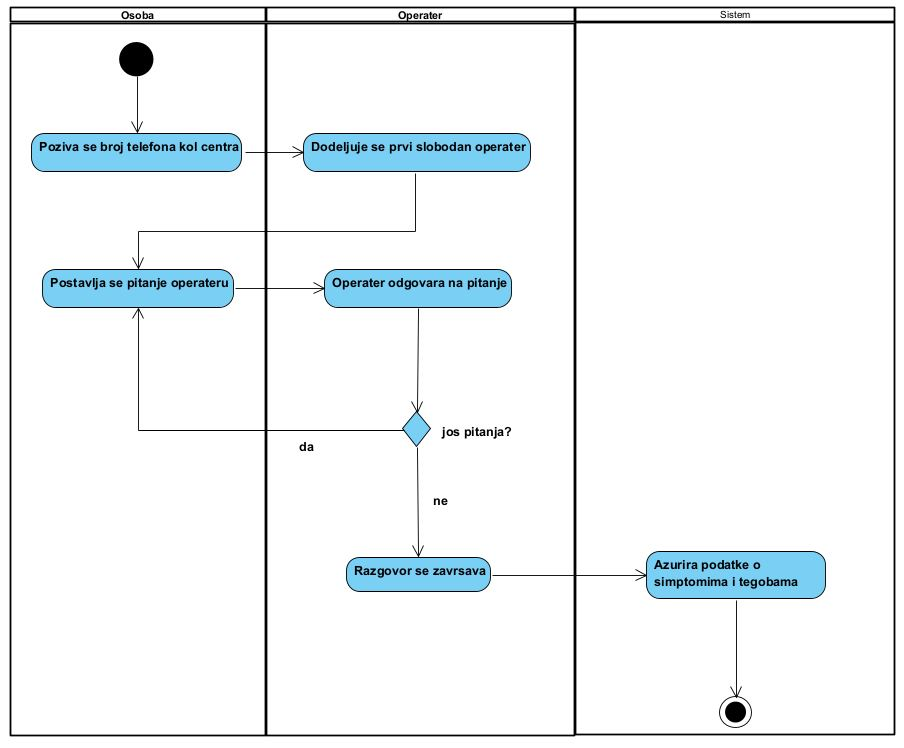
\includegraphics[scale=0.8]{Kol_centar}
\caption{Dijagram aktivnosti - Kol centar}
\end{figure}

\subsection{Kovid propusnice}

U ovom poglavlju se bavimo formalizacijom rada sa kovid propusnicama. U nastavku su opisani slučajevi upotrebe izdavanja i validacije kovid propusnica.

\subsubsection{Slučaj upotrebe: Izdavanje kovid propusnice}

%Prvih 5 tacaka je obavezno, ostale nisu - navesti potrebne
%Ne bi bilo loše da, ako se dodaje neki dijagram, stoji opis uz njega i da se negde u tekstu onda reveriše na tu sliku

\begin{itemize}
    \item \textbf{Kratak opis:} Registrovana osoba bira opciju za podnošenje zahteva za kovid propusnicu. Sistem proverava podatke, izdaje propusnicu i vraća odgovarajuću poruku.
    \item \textbf{Učesnici:}
        \begin{itemize}
            \item Registrovana osoba - želi brzo da dobije kovid propusnicu uz minimalan broj koraka
        \end{itemize}
    \item \textbf{Preduslovi:} Sistem je aktivan. Osoba je registrovana i ima pristup internetu.
    \item \textbf{Postuslovi:} Sistem je izdao propusnicu registrovanoj osobi.
    \item \textbf{Osnovni tok:}
        \begin{enumerate}
            \item Osoba otvara stranicu za prijavu.
            \item Sistem prikazuje formular za prijavu.
            \item Osoba unosi odgovarajuće podatke.
            \item Osoba potvrđuje unos.
            \item Sistem vrši validaciju podataka.
            \item Osoba otvara stranicu za podnošenje zahteva za izdavanje propusnice.
            \item Sistem prikazuje tri moguće opcije:
                \begin{itemize}
                    \item Izdavanje propusnice na osnovu primljene vakcine.
                    \item Izdavanje propusnice na osnovu negativnog PCR ili antigenskog testa.
                    \item Izdavanje propusnice na osnovu preležanog virusa.
                \end{itemize}
            \item Osoba bira jednu od ponuđenih opcija.
            \item Sistem proverava zadovoljenost uslova.
            \item Sistem osobi šalje mejl sa kovid propusnicom.
            \item Sistem obaveštava osobu da je operaciju uspešno izvršena i da je propusnica poslata.
        \end{enumerate}
     
    %Ako postoje, podtokove nazivati sa P1, P2, ...   
    %\item \textbf{Podtokovi:}    
    
    %Alternativne tokove nazivati sa A1, A2, ...
    \item \textbf{Alternativni tokovi:}
        \begin{itemize}
            \item[A1.] \textbf{Neuspešno prijavljivanje.} Ukoliko u koraku 5 osnovnog toka sistem naiđe na neispravne podatke, obaveštava osobu i zahteva ponovni unos podataka. Proces se nastavlja u koraku 3 osnovnog toka.
            \item[A2.] \textbf{Uslovi za izdavanje nisu zadovoljeni.} Ukoliko u koraku 9 osnovnog toga sistem ustanovi da nisu zadovoljeni odgovarajući uslovi za izdavanje propusnice, obaveštava osobu. Proces se završava.
        \end{itemize}
    
    %Ako postoje, specijalne zahteve navesti ovde
    %\item \textbf{Specijalni zahtevi:}
        
    \item \textbf{Dodatne informacije:}
        \begin{itemize}
            \item Podaci koji su potrebni za prijavu na sistem su korisničko ime i lozinka.
            \item Uslovi za izdavanje propusnice su:
                \begin{itemize}
                    \item Druga doza vakcine je primljena pre manje od 7 meseci ili  je primljena treća doza vakcine.
                    \item Postojanje negativnog PCR testa koji nije stariji od 72 sata ili antigenskog testa koji nije stariji od 48 sati.
                    \item Virus je preležan pre manje od 7 meseci.
                \end{itemize}
            \item Kovid propusnica sadrži QR kod na osnovu kog se proverava validnost propusnice.
        \end{itemize}
\end{itemize}

\begin{figure}[H]
\centering
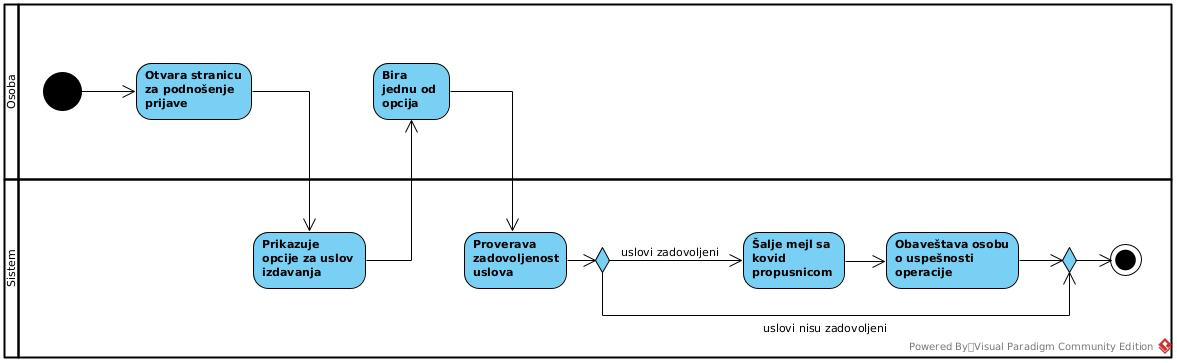
\includegraphics[scale=0.25]{Izdavanje_propusnice}
\caption{Dijagram aktivnosti - Izdavanje kovid propusnice}
\label{slk:izdavanje}
\end{figure}

\subsubsection{Slučaj upotrebe: Validacija kovid propusnica}

\begin{itemize}
    \item \textbf{Kratak opis:} Kontrolor očitava QR kod sa kovid propusnice. Sistem proverava podatke i prikazuje odgovarajuću poruku o validnosti propusnice.
    \item \textbf{Učesnici:}
        \begin{itemize}
            \item Kontrolor - želi brzo da proveri validnost kovid propusnice
        \end{itemize}
    \item \textbf{Preduslovi:} Sistem je aktivan. Kontrolor ima pristup internetu.
    \item \textbf{Postuslovi:} Sistem je obavestio kontrolora o validnosti kovid propusnice.
    \item \textbf{Osnovni tok:}
        \begin{enumerate}
            \item Kontrolor očitava QR kod sa kovid propusnice.
            \item Kontrolor otvara stranicu za validaciju.
            \item Sistem dobija zahtev za validaciju propusnice.
            \item Sistem proverava zadovoljenost uslova za važenje propusnice.
            \item Sistem prikazuje podatke o vlasniku propusnice i status propusnice:
                \begin{itemize}
                    \item Zeleno - ukoliko su uslovi za važenje propusnice zadovoljeni.
                    \item Crveno - ukoliko uslovi za važenje propusnice nisu zadovoljeni.
                \end{itemize}
        \end{enumerate}
    \item \textbf{Specijalni zahtevi:}
        \begin{itemize}
            \item Kontrolor poseduje uređaj kojim se može skenirati QR kod.
        \end{itemize}
    \item \textbf{Dodatne informacije:}
        \begin{itemize}
            \item Uslovi za važenje propusnice su:
                \begin{itemize}
                    \item Druga doza vakcine je primljena pre manje od 7 meseci ili  je primljena treća doza vakcine.
                    \item Postojanje negativnog PCR testa koji nije stariji od 72 sata ili antigenskog testa koji nije stariji od 48 sati.
                    \item Virus je preležan pre manje od 7 meseci.
                \end{itemize}
        \end{itemize}
\end{itemize}

\begin{figure}[H]
\centering
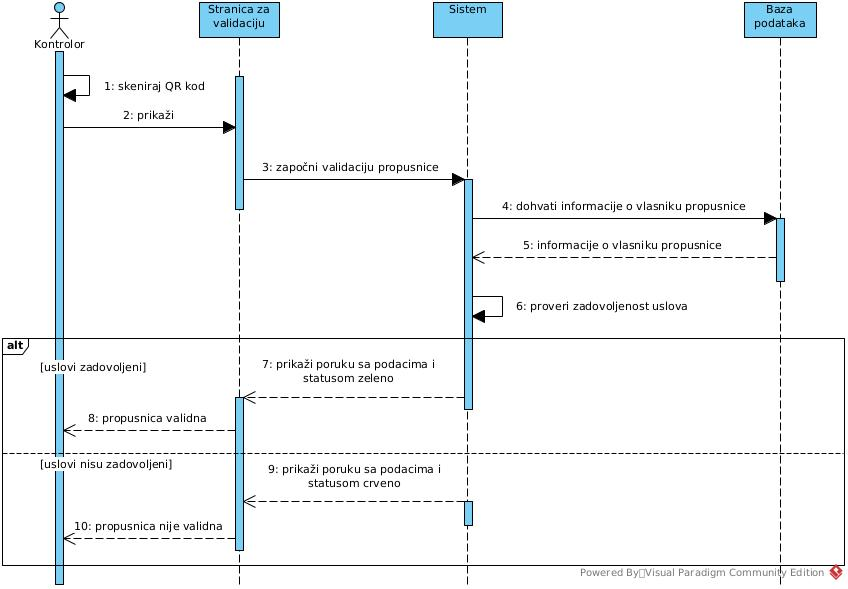
\includegraphics[scale=0.5]{Validacija_propusnice}
\caption{Dijagram sekvence - Validacija kovid propusnice}
\label{slk:validacija}
\end{figure}

\subsection{Testiranje}

\subsubsection{Slučaj upotrebe: Unos informacija o urađenom testu}

\end{document}
